\documentclass[11pt,letterpaper]{article}

\usepackage[utf8]{inputenc}
\usepackage{amsmath}
\usepackage{amsfonts}
\usepackage{amssymb}
\usepackage{fancyhdr}
\usepackage{graphicx}
\usepackage{listings}% http://ctan.org/pkg/listings
\usepackage{xcolor}
\usepackage{hyperref}
\usepackage{pdfpages}

\definecolor{codegreen}{rgb}{0,0.6,0}
\definecolor{codegray}{rgb}{0.5,0.5,0.5}
\definecolor{codepurple}{rgb}{0.58,0,0.82}
\definecolor{backcolour}{rgb}{0.95,0.95,0.92}
\lstdefinestyle{mystyle}{
    backgroundcolor=\color{backcolour},   
    commentstyle=\color{codegreen},
    keywordstyle=\color{magenta},
    numberstyle=\tiny\color{codegray},
    stringstyle=\color{codepurple},
    basicstyle=\ttfamily\footnotesize,
    breakatwhitespace=false,         
    breaklines=true,                 
    captionpos=b,                    
    keepspaces=true,                 
    numbers=left,                    
    numbersep=5pt,                  
    showspaces=false,                
    showstringspaces=false,
    showtabs=false,
    tabsize=2
}

\hypersetup{
    colorlinks=true,
    linkcolor=blue,
    filecolor=magenta,      
    urlcolor=cyan,
}

\lstset{style=mystyle}

\pagestyle{fancy}
\fancyhf{}
\lhead{\footnotesize{Design Document: MT rpcserver}}
\rhead{\footnotesize{Perry David Ralston Jr. CruzID: pdralsto}}
\cfoot{\footnotesize{Page \thepage}}


\title{Design Document: multi-threaded rpcserver}
\author{Perry David Ralston Jr.\\ CruzID: pdralsto}

\begin{document}
\maketitle
\thispagestyle{fancy}
\section{Goals}

This multi-threaded RPC Server will build off of the design of the previous RPC server. The design for the origianl RPC Server can be found at the end of this document. The design from there remains unchanged unless specifically called out in this design document. The goal of this project is to create an RPC server capable of handling simultaneous requests from numerous clients, leveraging the synchronization techniques learned in lecture. Noted additions to this server is the dispatch thread, responsible for assigning worker threads to the inbound connections, and a shared key-value store for managing the store of variable values that all of the threads can access and modify in a semi-volatile manner. The key-value store persists across all connections to the server and is readable/editable by any thread with coordination.

\section{Hash Table}

For this project, I will be reviving and heavily modifying a hash table that I coded in March of 2017. The key structure of the hash table is a fixed size array of Node*(s) that make up a linked list. The nodes themselves contain a name stored as a char* and a value, int64\_t. The hashing is done using a basic hashing function with a fixed decimal constant. The hash table supports the following public functions: insert, replace, delete, clear, dump, and load. The algorithims are detailed below. This hash table implements synchronized access on the index level by implementing a parallel array of semaphores that the neccesary functions will wait and signal on. Calls to this synchronized hash table requires a thread to send their unique identifier to facilitate node level access within a bucket the thread already acquired a lock on.

\subsection{Node Structure and Functions}

Nodes are structured as a key value pair with a pointer to the next node in the list. Nodes are inserted into the hash table by hashing their key to acquire the index for the list that they will be inserted into. See diagram below.

\begin{center}
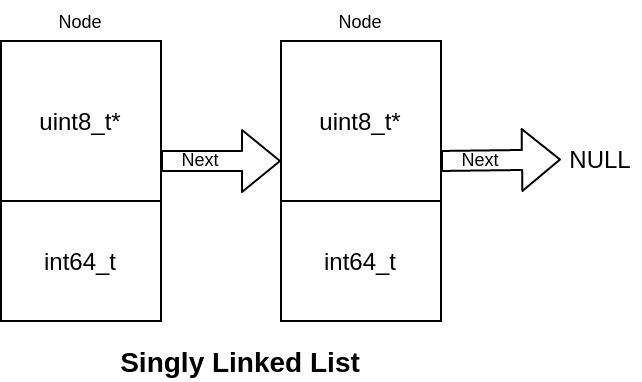
\includegraphics[scale=.4]{node.jpg}
\end{center}

\subsection{Hash Table Functions}
\begin{center}
\lstinputlisting[language=Python, frame=single]{hashing_function}
\textbf{\footnotesize{Hashing Function}}
\end{center}
\begin{minipage}{\linewidth}
\begin{center}
\lstinputlisting[language=Python, frame=single]{insert}
\textbf{\footnotesize{Insert}}
\end{center}
\end{minipage}
\begin{center}
\lstinputlisting[language=Python, frame=single]{replace}
\textbf{\footnotesize{Replace}}
\end{center}
\begin{center}
\lstinputlisting[language=Python, frame=single]{delete}
\textbf{\footnotesize{Remove}}
\end{center}
\begin{minipage}{\linewidth}
\begin{center}
\lstinputlisting[language=Python, frame=single]{lookup}
\textbf{\footnotesize{Lookup}}
\end{center}
\end{minipage}
\begin{center}
\lstinputlisting[language=Python, frame=single]{clear}
\textbf{\footnotesize{Clear}}
\end{center}
\begin{center}
\lstinputlisting[language=Python, frame=single]{save}
\textbf{\footnotesize{Dump}}
\end{center}
\begin{minipage}{\linewidth}
\begin{center}
\lstinputlisting[language=Python, frame=single]{load}
\textbf{\footnotesize{Load}}
\end{center}
\end{minipage}

\section{Multi-Threading}

In the previous rpcserver, request handling was limited to a single request at a time. Using the shared hash table described above and the pthread library, this rpcserver will have the ability to servce -N clients at the same time. -N is a command line argument that denotes the number of threads that the server should initially service. The default N value is 4. To achieve this, a structure will be created to house the thread references and act as a means of communication between the dispatch thread and the worker threads. The over all design is pictured below:
\begin{center}
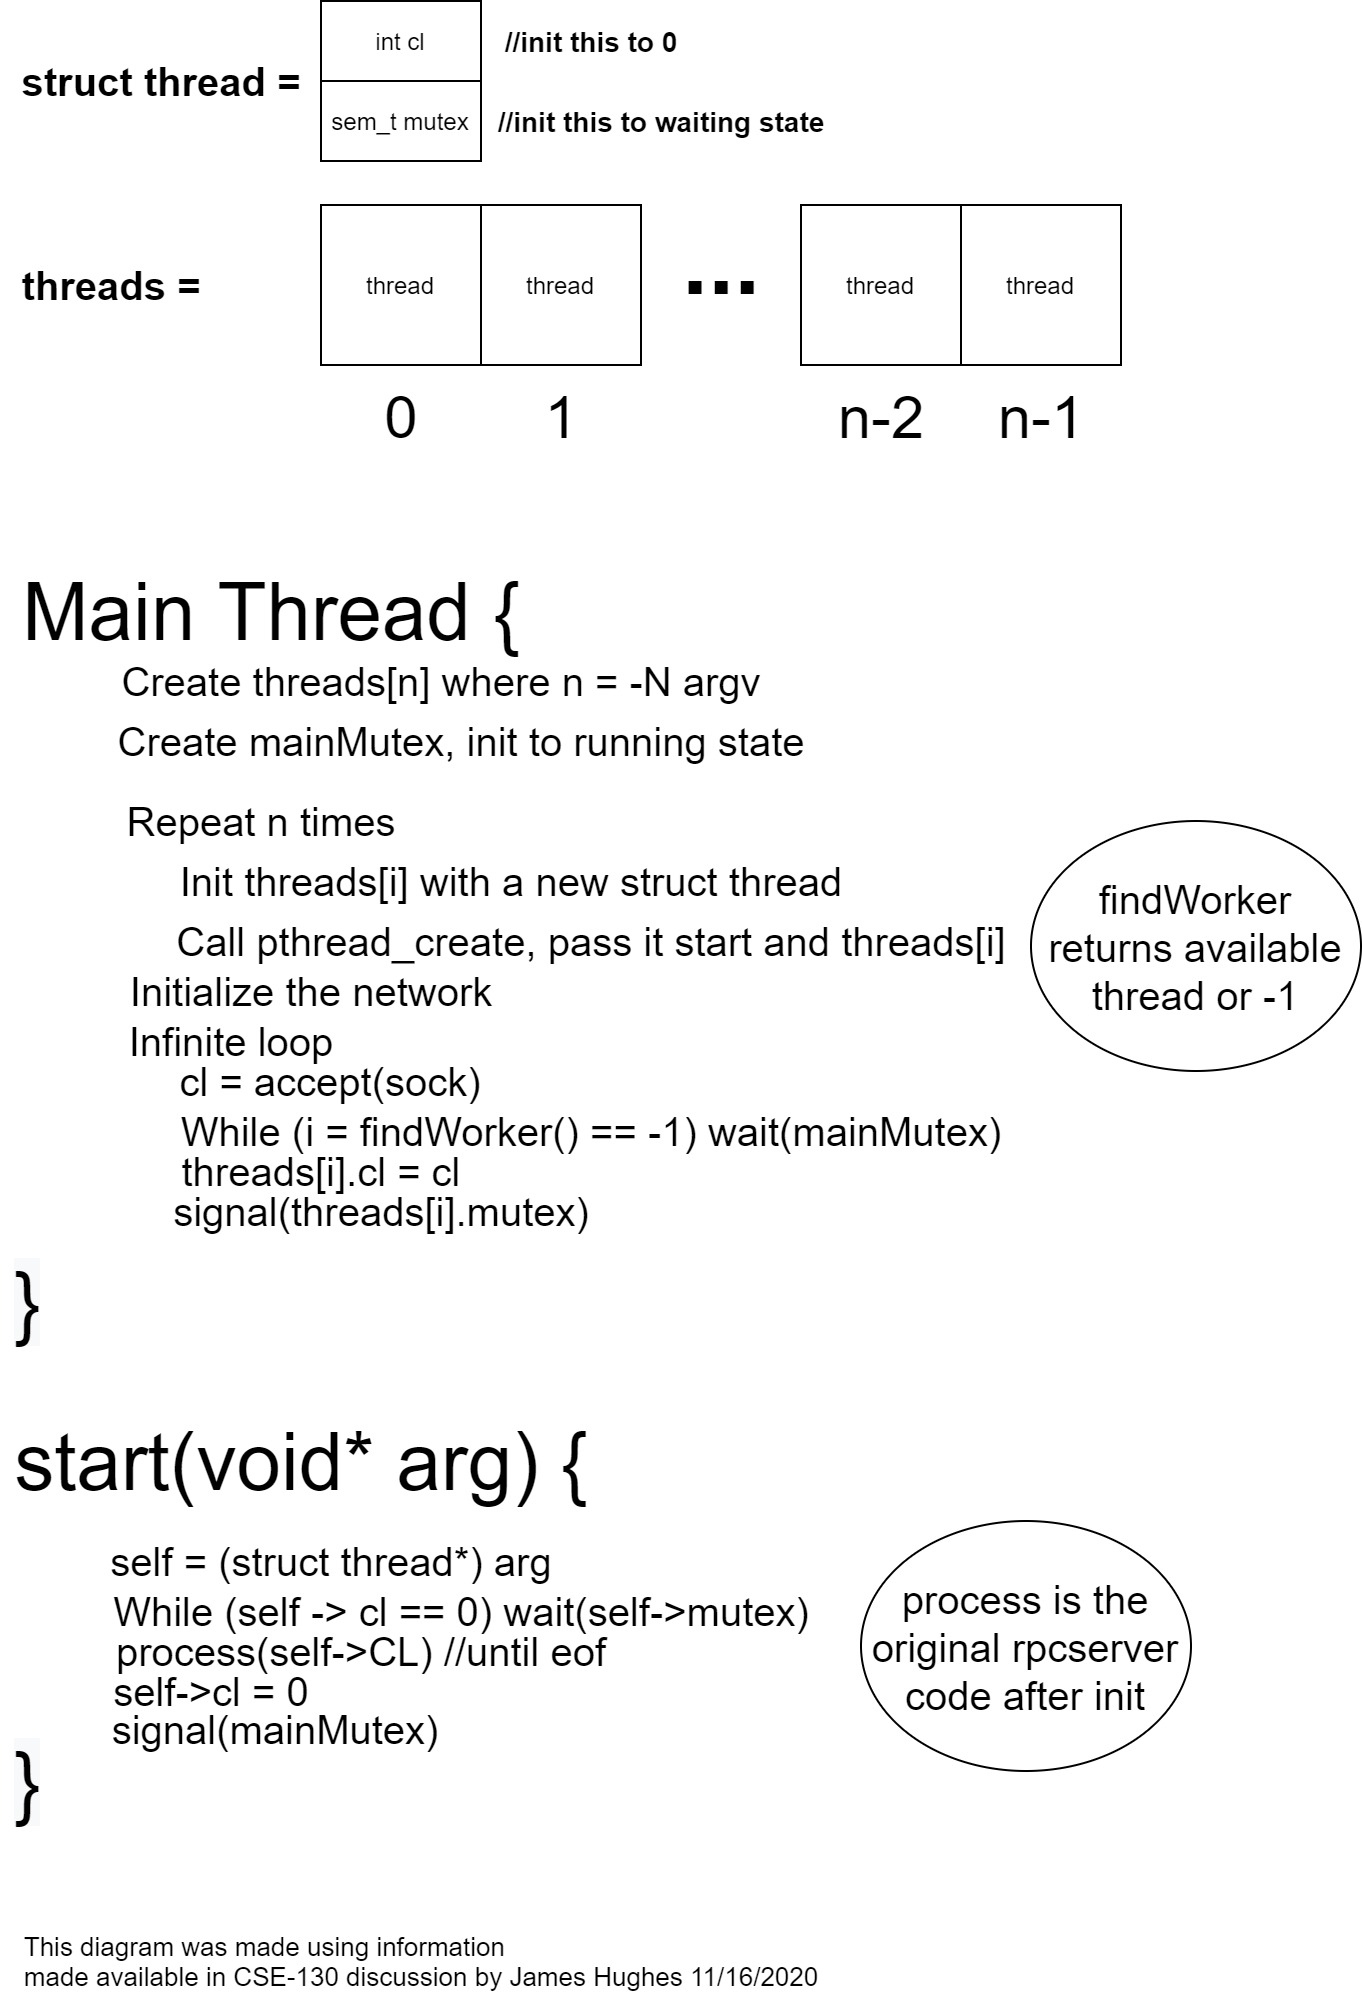
\includegraphics[scale=.2]{threads.jpg}
\end{center}

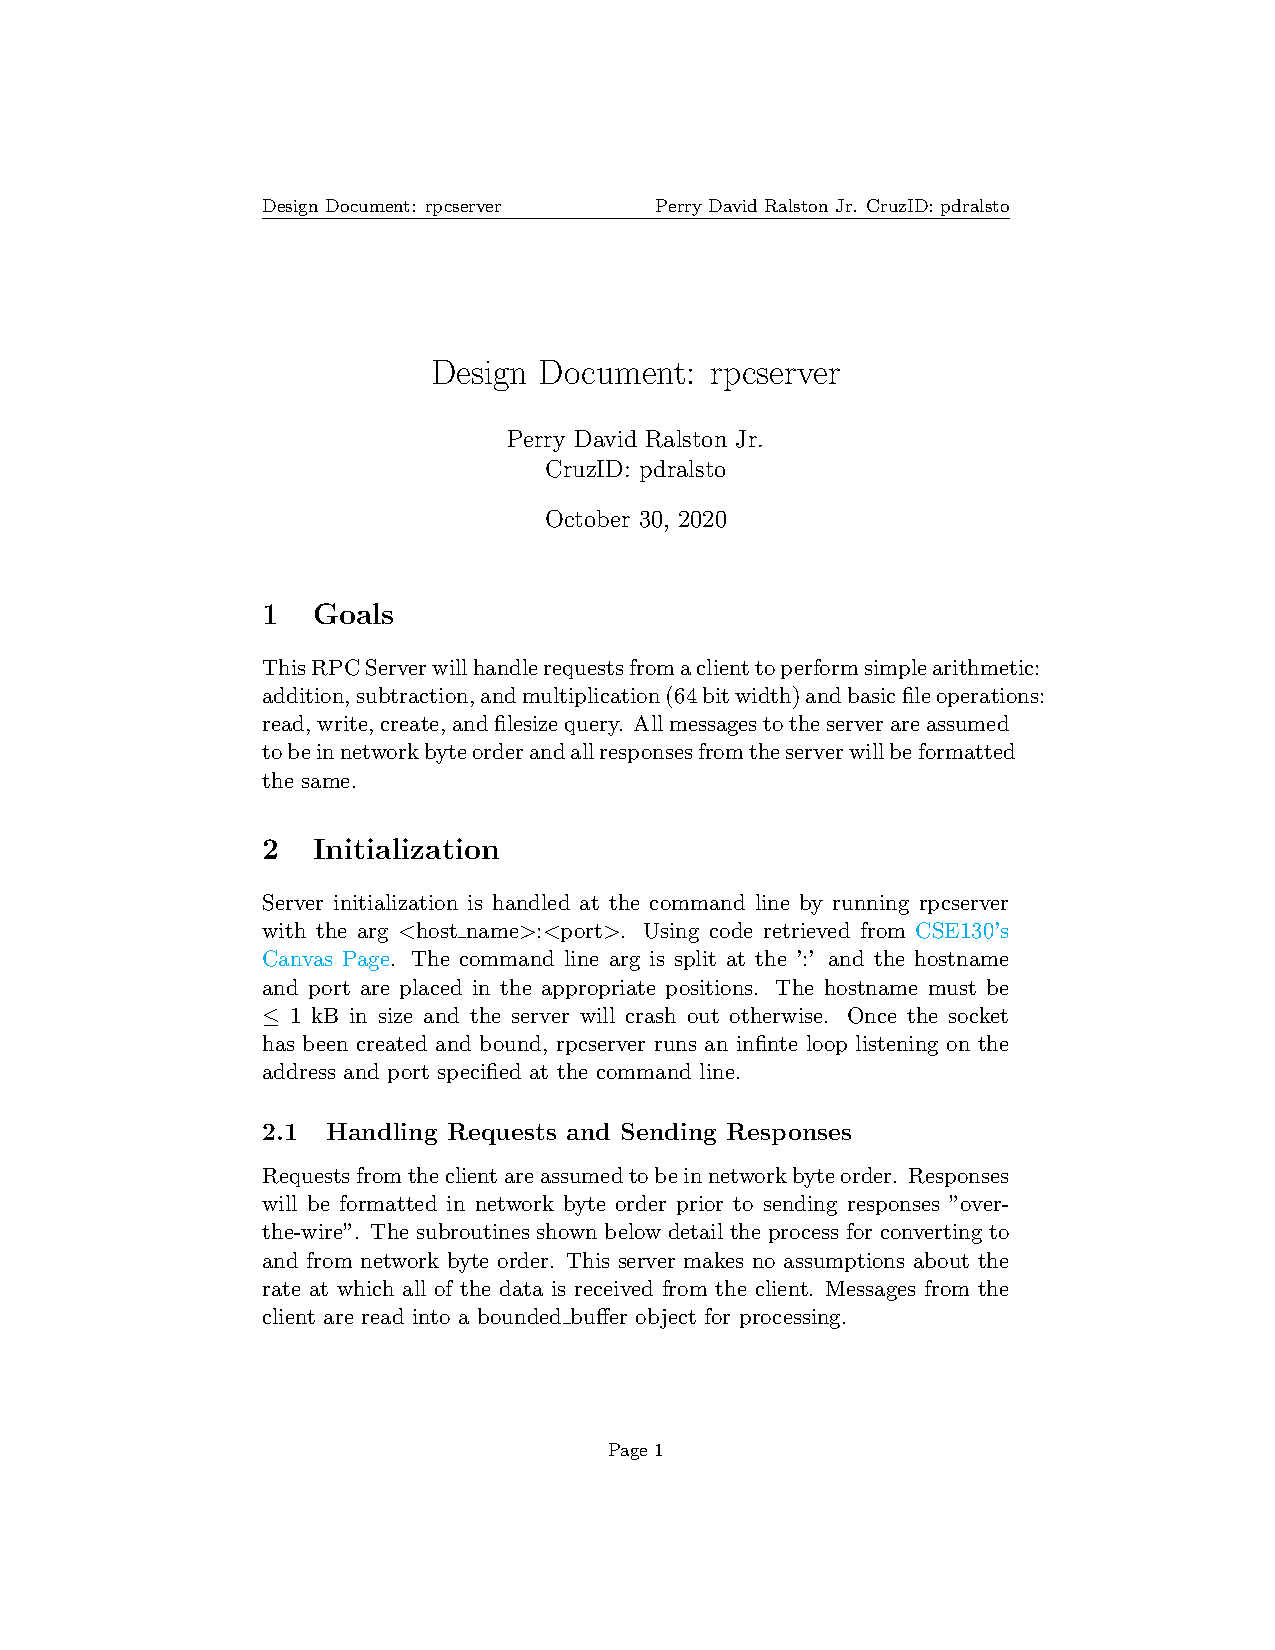
\includepdf[pages={-}]{PREV_DESIGN.pdf}
\end{document}